\documentclass[]{beamer}
\usepackage[T1]{fontenc}
\usepackage[utf8]{inputenc}
\usepackage{lmodern}
\usepackage[italian]{babel}
\usepackage{mathrsfs}

\title{Flusso e circuitazione di un campo}
\author{\texorpdfstring{Mattia Cozzi\newline\href{mailto:cozzimattia@gmail.com}{\texttt{cozzimattia@gmail.com}}}{Mattia Cozzi}}
\date{a.s.~2023/2024}

%\documentclass[handout]{beamer}     %usare questa classe per generare l'handout
%\usepackage{pgfpages}   %per mostrare più quadri nella stessa pagina
%\pgfpagesuselayout{4 on 1}[a4paper,border shrink=5mm,landscape]
\usetheme{Singapore}
%\useoutertheme[left]{sidebar} %elementi intorno alle diapositive
\setbeamercovered{dynamic} %modifica l'aspetto del testo grigetto delle diapositive future. Argomenti: invisible/transparent/dynamic
\usecolortheme{orchid}
%COLORE PRINCIPALE
% \definecolor{marroncino}{RGB}{156, 26, 0} % UBC Blue (primary)
% \setbeamercolor{structure}{fg=marroncino} % itemize, enumerate, etc

\theoremstyle{plain}
\newtheorem{teorema}{Teorema}

\usepackage{tikz}
\usepackage{circuitikz}

\usepackage{pgf,pgfplots,graphicx}
\usetikzlibrary{angles,quotes,arrows,shapes,decorations.markings}
\pgfplotsset{compat=1.15}
\usepgfplotslibrary{units,fillbetween} % to add units easily to axis

\newcommand{\fem}{f_{em}}

\def\angolo[#1](#2)(#3:#4:#5)% Syntax: [draw options] (center) (initial angle:final angle:radius)
    { \draw[#1] ($(#2)+({#5*cos(#3)},{#5*sin(#3)})$) arc (#3:#4:#5); }


\begin{document}

\begin{frame}
  \titlepage
\end{frame}





\begin{frame}
\frametitle{Contenuti}
\tableofcontents
\end{frame}

\section{Introduzione}

\begin{frame}
\frametitle{Moto dei fluidi}
  I due concetti che qui trattiamo, \alert{flusso} e \alert{circuitazione} di un campo, sono stati originariamente introdotti in fisica relativamente alla meccanica nei fluidi (parlando di vettori velocità delle particelle e non di vettori campo).\\Sarà utile tenere questa idea come riferimento, soprattutto nel caso del flusso.
\end{frame}



\begin{frame}
\frametitle{Prodotto scalare}
Entrambe le quantità vengono introdotte mediante un \alert<1>{prodotto scalare tra due vettori $ \vec{a} $ e $ \vec{b} $}, che si calcola come:
  \begin{center}
  $ \vec{a} \cdot \vec{b} = a b \cos\theta $
  \end{center}
  con $ \theta $ angolo tra i due vettori.\\\pause~\\
  Intuitivamente, il prodotto scalare permette di valutare ``quanto del vettore $ \vec{a} $ giace sul vettore $ \vec{b} $''.
\end{frame}


\begin{frame}
\frametitle{Vettore superficie}
\visible<1->{Introduciamo, per utilizzarlo poi nella definizione di flusso, il \emph{vettore superficie}. Data una superficie piana $ S $, esso ha:}
  \begin{itemize}
    \item \visible<2->{direzione perpendicolare a $ S $;}
    \item \visible<3->{modulo pari a $ S $.} 
  \end{itemize}
  
  \begin{figure}
\begin{tikzpicture}
\visible<1->{\fill[fill=red!20] (0,0) -- (4,0) -- (3,-1) -- (-1,-1) -- cycle;
\node [right,thick] at (2.5,0) {$ S $};}
\visible<2->{\draw [dashed] (1.5,-.5) -- (1.5,2.5);
\draw [dotted] (1.5,-1) -- (1.5,-.5);
\draw [dashed] (1.5,-1) -- (1.5,-1.5);}
\visible<3->{\node [right,blue,thick] at (1.5,1) {$ \vec{S} $};
\draw [->,blue,thick] (1.5,-.5) -- (1.5,2);}
\end{tikzpicture}
\end{figure}

\end{frame}




\section{Flusso di $ \vec{E} $}

\begin{frame}
  \frametitle{Flusso del campo elettrico}
Il flusso del campo elettrico è definito come il prodotto scalare tra il campo elettrico $ \vec{E} $ che attraversa la superficie $ S $ e il vettore superficie $ \vec{S} $ definito sopra.
\begin{center}
   \colorbox{blue!30}{$ \Phi_{S}(\vec{E}) = \vec{E} \cdot \vec{S} = ES\cos\theta $}
\end{center}
\begin{figure}
\begin{tikzpicture}
\fill[fill=red!20] (0,0) -- (4,0) -- (3,-1) -- (-1,-1) -- cycle;
\angolo[black](1.5,-.5)(52:90:.8)
\node [left,thick] at (2.1,.6) {$ \theta $};
\node [left,blue,thick] at (1.5,1) {$ \vec{S} $};
\draw [->,blue,thick] (1.5,-.5) -- (1.5,2);
\node [left,red,thick] at (3.3,1) {$ \vec{E} $};
\draw [->,red,thick] (1.5,-.5) -- (3,1.5);
\end{tikzpicture}
\end{figure}
\end{frame}

\begin{frame}
  \frametitle{Il ruolo dell'angolo}



\begin{columns}
\begin{column}{0.5\textwidth}
\begin{figure}
\begin{tikzpicture}[scale=.5]
\fill[fill=red!20] (0,0) -- (4,0) -- (3,-1) -- (-1,-1) -- cycle;
\node [right,thick] at (1.5,.3) {{\tiny $ \theta $}};
\node [left,blue,thick] at (1.5,1) {{\tiny $ \vec{S} $}};
\draw [->,blue,thick] (1.5,-.5) -- (1.5,2);
\node [right,red,thick] at (1.5,1) {{\tiny $ \vec{E} $}};
\draw [->,red,thick] (1.5,-.5) -- (1.5,1.5);
\end{tikzpicture}

$ \cos\theta = 1 $\\flusso massimo
\end{figure}


\begin{figure}
\begin{tikzpicture}[scale=.5]
\fill[fill=red!20] (0,0) -- (4,0) -- (3,-1) -- (-1,-1) -- cycle;
\angolo[black](1.5,-.5)(52:90:.8)
\node [left,thick] at (2.2,.6) {{\tiny $ \theta $}};
\node [left,blue,thick] at (1.5,1) {{\tiny $ \vec{S} $}};
\draw [->,blue,thick] (1.5,-.5) -- (1.5,2);
\node [left,red,thick] at (3.5,1) {{\tiny $ \vec{E} $}};
\draw [->,red,thick] (1.5,-.5) -- (3,1.5);
\end{tikzpicture}

$ 0 < \cos\theta < 1 $\\flusso intermedio
\end{figure}
\end{column}
\begin{column}{0.5\textwidth}
\begin{figure}
\begin{tikzpicture}[scale=.5]
\fill[fill=red!20] (0,0) -- (4,0) -- (3,-1) -- (-1,-1) -- cycle;
\angolo[black](1.5,-.5)(0:90:.8)
\node [left,thick] at (2.2,.6) {{\tiny $ \theta $}};
\node [left,blue,thick] at (1.5,1) {{\tiny $ \vec{S} $}};
\draw [->,blue,thick] (1.5,-.5) -- (1.5,2);
\node [left,red,thick] at (3.5,0) {{\tiny $ \vec{E} $}};
\draw [->,red,thick] (1.5,-.5) -- (3,-.5);
\end{tikzpicture}

$ \cos\theta = 0 $\\flusso nullo
\end{figure}



\begin{figure}
\begin{tikzpicture}[scale=.5]
\fill[fill=red!20] (0,0) -- (4,0) -- (3,-1) -- (-1,-1) -- cycle;
\angolo[black](1.5,-.5)(0:90:.8)
\angolo[black,dotted](1.5,-.5)(-45:0:.8)
\node [left,thick] at (2.2,.6) {{\tiny $ \theta $}};
\node [left,blue,thick] at (1.5,1) {{\tiny $ \vec{S} $}};
\draw [->,blue,thick] (1.5,-.5) -- (1.5,2);
\node [left,red,thick] at (3.3,-1) {{\tiny $ \vec{E} $}};
\draw [red,thick,dotted] (1.5,-.5) -- (2,-1);
\draw [->,red,thick] (2,-1) -- (2.5,-1.5);
\end{tikzpicture}

$ -1 < \cos\theta < 0 $\\flusso negativo
\end{figure}
\end{column}
\end{columns}
\end{frame}

\begin{frame}
  \frametitle{Superficie chiusa}
  \begin{block}{Definizione}
    Una superficie chiusa (o gaussiana) è una superficie che racchiude un volume.
  \end{block}\pause~\\
  Sono esempi di superfici chiuse la plastica di un palloncino o le pareti di una bottiglia tappata.
\end{frame}





\begin{frame}
  \frametitle{Flusso attraverso una superficie chiusa (1)}
  Per calcolare il flusso attraverso una superficie chiusa $ S $ dobbiamo:
  \begin{itemize}
    \item dividere la superficie in $ n $ parti (al limite infinite) ognuna così piccola da poterla considerare \alert<1>{piana} e \alert<1>{uniforme} il campo elettrico attraverso di essa;\pause
    \item indicare con $ \Delta \vec{S}_i $ il \alert<2>{vettore superficie} associato alla porzione di superficie $ S_i $;\pause
    \item determinare il vettore $ \vec{E}_i $, cioè il \alert<3>{campo elettrico attraverso $ \Delta \vec{S}_i $};\pause
    \item calcolare il \alert<4>{prodotto scalare} $ \vec{E}_i \cdot \Delta \vec{S}_i $.
  \end{itemize}
\end{frame}

\begin{frame}
  \frametitle{Flusso attraverso una superficie chiusa (2)}
  Il flusso totale attraverso la superficie $ S $ sarà la \alert<1>{somma di tutti i prodotti scalari}, calcolati per ogni sezione di $ S $.
   \begin{center}
   \colorbox{blue!30}{$ \Phi_S (\vec{E}) = \sum\limits_{i=1}^n \vec{E}_i \cdot \Delta \vec{S}_i =  \sum\limits_{i=1}^n E_i \Delta S_i \cos\theta_i $}
   \end{center}
\end{frame}




\begin{frame}
  \frametitle{Il teorema di Gauss per il campo elettrico}
  Per il flusso di $ \vec{E} $ vale il seguente teorema.
  \begin{block}{Teorema di Gauss per il campo elettrico}
    Il flusso del campo elettrico attraverso una superficie chiusa (gaussiana) è direttamente proporzionale alla carica totale contenuta all'interno della superficie.
    \begin{center}
   \colorbox{blue!30}{$ \Phi_S (\vec{E}) = \dfrac{Q_{tot}}{\varepsilon_0} $}
   \end{center}
  \end{block}\pause
  Il valore del flusso non dipende dalla specifica superficie o da come è distribuita la carica all'interno di essa.
\end{frame}




\section{Flusso di $ \vec{B} $}



\begin{frame}
  \frametitle{Flusso  del campo magnetico}
  Il flusso di $ \vec{B} $ attraverso una superficie $ S $ (eventualmente gaussiana) si definisce in modo analogo a quello di $ \vec{E} $. 
  \begin{center}
   \colorbox{blue!30}{$ \Phi_{S}(\vec{B}) = \vec{B} \cdot \vec{S} = BS\cos\theta $}
\end{center}\pause
Il flusso del campo magnetico si misura in \emph{weber}:
\begin{center}
$ [Wb] = [T\cdot m^2] $
\end{center}
\end{frame}




\begin{frame}
  \frametitle{Il teorema di Gauss per il campo magnetico}
  Per il flusso di $ \vec{B} $ vale il seguente teorema.
  \begin{block}{Teorema di Gauss per il campo magnetico}
    Il flusso del campo magnetico attraverso una superficie chiusa (gaussiana) è uguale a zero.
    \begin{center}
   \colorbox{blue!30}{$ \Phi_S (\vec{B}) = 0 $}
   \end{center}
  \end{block}\pause
  Mentre esistono cariche elettriche isolate, non esistono monopòli magnetici (poli nord o sud isolati): abbiamo sempre lo stesso numero di poli nord e sud magnetici, ovvero \alert{per ogni linea di campo uscente ci sarà una linea di campo entrante}.
\end{frame}


\section{Circuitazione di $ \vec{E} $}



\begin{frame}
  \frametitle{La circuitazione del campo elettrostatico (1)}
  Per calcolare la circuitazione del campo $ \vec{E} $ occorre scegliere arbitrariamente una linea chiusa e orientata $ \mathscr{L} $ e:\pause
  \begin{itemize}
    \item dividerla in $ n $ parti (al limite infinite) ognuna così piccola da poterla considerare \alert<2>{rettilinea} e \alert<2>{uniforme} il campo elettrico lungo di essa;\pause
    \item indicare con $ \Delta \vec{\ell}_i $ il \alert<3>{vettore spostamento} che descrive il tratto numero $ i $ di $ \mathscr{L} $;\pause
    \item determinare il vettore $ \vec{E}_i $, cioè il \alert<4>{campo elettrico lungo $ \Delta \vec{\ell}_i $};\pause
    \item calcolare il \alert<5>{prodotto scalare} $ \vec{E}_i \cdot \Delta \vec{\ell}_i $.
  \end{itemize}
\end{frame}


\begin{frame}
  \frametitle{La circuitazione del campo elettrostatico (2)}
  \begin{figure}
  \begin{tikzpicture}[xscale=.8,yscale=.8]
\draw [purple, thick] (0,0) circle [radius=3];
\angolo[black](7.5,1)(270:307:1)
\node [left, purple] at (-2.5,2) {$ \mathscr{L} $};
\draw (3,0) circle [radius=.2];
\draw (3,.2) -- (6.8,1.875);
\draw (3,-.2) -- (6.8,-1.875);
\draw (7.5,0) circle [radius=2];
\draw [thick, purple] (7.5,2)  -- (7.5,-2);
\draw [thick, blue, ->] (7.5,1)  -- (9,-1);
\node [left, purple] at (7.5,0) {{\scriptsize $ \Delta\vec{\ell}_i $}};
\node [right, blue] at (7.8,.8) {{\scriptsize $ \vec{E}_i $}};
\node [below] at (7.9,0.1) {{\scriptsize $ \theta_i $}};
\draw [thick, purple, ->] (-3,0)  -- (-3,.0001);
\end{tikzpicture}
\end{figure}
\begin{center}
   \colorbox{blue!30}{$ \Gamma_{\ell_i} (\vec{E}_i) = \vec{E}_i \cdot \Delta \vec{\ell}_i = E_i \ell_i \cos \theta_i $}
   \end{center}
\end{frame}




\begin{frame}
  \frametitle{La circuitazione lungo $ \mathscr{L} $}
  La circuitazione sarà la \alert<1>{somma di tutti i prodotti scalari}, calcolati per ogni tratto della linea $ \mathscr{L} $.
   \begin{center}
   \colorbox{blue!30}{$ \Gamma_\mathscr{L} (\vec{E}) = \sum\limits_{i=1}^n \vec{E}_i \cdot \Delta \vec{\ell}_i =  \sum\limits_{i=1}^n E_i \Delta \ell_i \cos\theta_i $}
   \end{center}
\end{frame}


\begin{frame}
  \frametitle{Il significato della circuitazione di $ \vec{E} $}
  Sappiamo che $ \vec{E}\cdot \Delta\vec{\ell} = - \Delta V $ e, indicando con $ \Delta V_i $  la differenza di potenziale tra gli estremi del segmento orientato $ \Delta \vec{\ell}_i $, avremo:
  \begin{center}
  $ \Gamma_\mathscr{L} (\vec{E}) = \sum\limits_{i=1}^n \vec{E}_i \cdot \Delta \vec{\ell}_i = \sum\limits_{i=1}^n (-\Delta V_i) = - \sum\limits_{i=1}^n \Delta V_i = 0 $
  \end{center}
  La sommatoria delle differenze di potenziale lungo una linea chiusa è sempre nulla (legge delle maglie).\\\pause~\\
  
Ciò esprime matematicamente la proprietà del campo elettrostatico di essere \alert{conservativo}: il lavoro fatto dalla forza elettrica per spostare una carica non dipende dal percorso scelto ma solo dal punto di inizio e di fine (vale solo per il caso statico).
\end{frame}







\section{Circuitazione di $ \vec{B} $}

\begin{frame}
  \frametitle{Circuitazione del campo magnetico}
  La circuitazione di $ \vec{B} $ lungo un cammino orientato $ \mathscr{L} $ si definisce in modo analogo a quella di $ \vec{E} $. 
  \begin{center}
   \colorbox{blue!30}{$ \Gamma_\mathscr{L} (\vec{B}) = \sum\limits_{i=1}^n \vec{B}_i \cdot \Delta \vec{\ell}_i =  \sum\limits_{i=1}^n B_i \Delta \ell_i \cos\theta_i $}
   \end{center}
\end{frame}


\begin{frame}
\frametitle{Teorema di Ampère}
\begin{columns}
\begin{column}{0.5\textwidth}
Per $ \Gamma_B $ si dimostra che vale il \alert<1>{teorema di Ampère}, per cui:
\begin{center}
\colorbox{blue!30}{$ \Gamma_\mathscr{L} (\vec{B}) = \mu_0 \sum\limits_{k=1}^n i_k $}
\end{center}
dove $ i_k $ indica le $ k $ correnti concatenate a $ \mathscr{L} $.\pause
\end{column}
\begin{column}{0.4\textwidth}
\begin{figure}
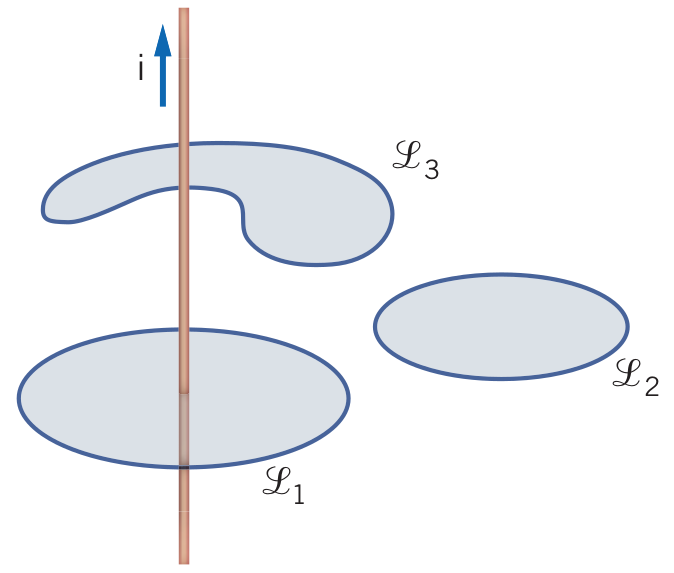
\includegraphics[width=\columnwidth]{img/teoremaampere.png}
\end{figure}
\end{column}
\end{columns}

~

~
   
Poiché il teorema di Ampère stabilisce che la circuitazione del campo magnetico può essere diversa da zero, affermiamo che, contrariamente al campo elettrostatico, \alert<2>{il campo magnetico non è conservativo}.
\end{frame}

\begin{frame}
  \frametitle{Dimostrazione della legge di Biot-Savart}
  La legge di Biot-Savart, che fornisce l'intensità del campo magnetico a distanza $ r $ da un filo rettilineo percorso da corrente, è un caso particolare del teorema di Ampère.\pause
  \begin{center}
  $ \Gamma_\mathscr{L} (\vec{B}) = \sum\limits_{i=1}^n \vec{B}_i \cdot \Delta \vec{\ell}_i = B \sum\limits_{i=1}^n \Delta \ell_i = B 2 \pi r = \mu_0 i $
  \end{center}
  da cui:
    \begin{center}
   \colorbox{blue!30}{$ B = \mu_0 \dfrac{i}{2\pi r} $}
   \end{center}
\end{frame}



\section{Equazioni (1)}

\begin{frame}
\frametitle{Le equazioni di Maxwell (caso statico)}
  Riassumiamo quanto detto con le \alert{quattro equazioni di Maxwell} per il caso statico:\pause
\begin{enumerate}
  \item Teorema di Gauss per il campo elettrico
  \begin{center}
  \colorbox{blue!30}{$ \Phi_S (\vec{E}) = \dfrac{Q_{tot}}{\varepsilon_0} $}
  \end{center}\pause
  \item Teorema di Gauss per il campo magnetico
  \begin{center}
  \colorbox{blue!30}{$ \Phi_S (\vec{B}) = 0 $}
  \end{center}\pause
  \item Legge di FNL (per il campo elettrostatico)
  \begin{center}
\colorbox{blue!30}{  $ \Gamma_\mathscr{L} (\vec{E}) = 0 $}
  \end{center}\pause
  \item Teorema di Ampère
  \begin{center}
  \colorbox{blue!30}{$ \Gamma_\mathscr{L} (\vec{B}) = \mu_0 \sum\limits i_k $}
  \end{center}
\end{enumerate}
\end{frame}

\begin{frame}
  \frametitle{1.~Il teorema di Gauss per $ \vec{E} $}
    \begin{center}
  \colorbox{blue!30}{$ \Phi_S (\vec{E}) = \dfrac{Q_{tot}}{\varepsilon_0} $}
  \end{center}\pause
  Dice che:
  \begin{itemize}
    \item le linee del campo elettrico possono essere aperte;\pause
    \item esistono cariche elettriche isolate;\pause
    \item le cariche sono le sorgenti del campo elettrico.
  \end{itemize}
\end{frame}

\begin{frame}
  \frametitle{2.~Il teorema di Gauss per $ \vec{B} $}
    \begin{center}
  \colorbox{blue!30}{$ \Phi_S (\vec{B}) = 0 $}
  \end{center}\pause
  Dice che:
  \begin{itemize}
    \item per ogni linea di campo entrante c'è una linea di campo uscente, ovvero tutte le linee del campo magnetico sono chiuse;\pause
    \item non esistono poli magnetici isolati.
  \end{itemize}
\end{frame}

\begin{frame}
  \frametitle{3.~La legge di Faraday-Neumann-Lenz}
  \begin{center}
\colorbox{blue!30}{  $ \Gamma_\mathscr{L} (\vec{E}) = 0 $}
  \end{center}\pause
  È la legge delle maglie e dice che:
  \begin{itemize}
    \item il campo elettrostatico è conservativo.
  \end{itemize}
\end{frame}

\begin{frame}
  \frametitle{4.~Il teorema di Ampère}
  \begin{center}
\colorbox{blue!30}{$ \Gamma_\mathscr{L} (\vec{B}) = \mu_0 i_k $}
  \end{center}\pause
  Dice che:
  \begin{itemize}
    \item il campo magnetico non è conservativo;\pause
    \item le cariche in moto (le correnti) sono le sorgenti del campo magnetico.
  \end{itemize}
\end{frame}



\end{document}
